\documentclass{article}
\usepackage[T2A]{fontenc}      
\usepackage[utf8]{inputenc}   
\usepackage[russian]{babel}   
\usepackage{graphicx}          
\usepackage{booktabs}          
\usepackage{geometry}
\geometry{margin=2.2cm}
\usepackage[hidelinks]{hyperref}


\title{Анализ и визуализация патентных данных}
\author{Твердюк Дмитрий ИУ6-13М}
\date{December 2025}

\begin{document}

\maketitle

\begin{abstract}
В работе рассматривается мини-проект по анализу и визуализации патентных данных USPTO с использованием семантических эмбеддингов PatentSBERTa, построенных по названиям изобретений. Цель исследования --- проверить, согласуются ли представления документов в векторном пространстве с технологической классификацией CPC, а также оценить влияние снижения размерности на результаты анализа. В рамках работы выполнено формирование генеральной совокупности по временным ограничениям, исследована структура данных по секциям и подсемействам CPC, проведено снижение размерности методом PCA на основе анализа кумулятивной объяснённой дисперсии, выполнена визуализация t-SNE для проверки локальной смысловой структуры и проведена количественная проверка гипотезы методом k ближайших соседей (kNN) с кросс-валидацией. Полученные результаты используются для обоснования применимости подхода в задачах семантического поиска, визуализации и мониторинга изменений патентного ландшафта.
\end{abstract}

\tableofcontents
\newpage

\section{Введение}
Патентные документы являются одним из наиболее полных источников технической информации и позволяют исследовать технологические тренды, выявлять близкие решения (prior art), строить технологические ландшафты, а также анализировать специализацию компаний и научных коллективов.
В рамках данного мини-проекта рассматривается прототип программной системы анализа и визуализации патентных данных USPTO, использующий семантические эмбеддинги PatentSBERTa по названиям изобретений. Семантические представления позволяют сравнивать документы по смыслу и выполнять поиск, кластеризацию и классификацию в едином векторном пространстве.

\section{Постановка задачи}
\subsection{Гипотеза исследования}
\textbf{H1:} эмбеддинги PatentSBERTa, построенные по \textbf{названиям} патентных документов, сохраняют семантическую структуру технологических подсемейств совместной патентной классификации (Cooperative Patent Classification, CPC). 
Структура проявляется в локальном соседстве (kNN) и в визуализации (t-SNE). 
При снижении размерности методом PCA до \textbf{186 компонент} (близко к уровню, при котором объясняется $\approx 90\%$ дисперсии) качество разделимости классов и локальных соседств \textbf{существенно не ухудшается}.

\subsection{Значимость исследования}
Основной целью создания программной системы анализа патентных данных является \textbf{автоматизированное прогнозирование изменений патентного ландшафта}: выявление развивающихся областей, фиксация появления новых тематических направлений, обнаружение \textbf{сближения/слияния технических областей} и иных структурных изменений.

Полученные результаты важны для разработки такой системы по следующим причинам:
\begin{itemize}
  \item \textbf{Прогнозирование динамики ландшафта:} если эмбеддинги устойчиво отражают технологические подсемейства CPC, то по изменению плотностей, ``центров'' и границ кластеров во времени можно отслеживать появление новых направлений, перераспределение фокусов и признаки слияния областей.
  \item \textbf{Семантический поиск и рекомендации:} высокая согласованность ближайших соседей с CPC-подсемействами означает, что по эмбеддингам можно эффективно находить ``похожие'' патенты и рекомендовать аналоги, что является базовой операцией при мониторинге технологий.
  \item \textbf{Автоматическая классификация:} простая модель kNN показывает способность восстанавливать технологические классы без использования полного текста (только по названиям), что полезно как быстрый baseline и как компонент пайплайна разметки/проверки качества данных.
  \item \textbf{Ускорение и масштабируемость (оптимизация вычислений):} PCA-редукция почти не снижает качество, но уменьшает размерность и вычислительные затраты, что критично для интерактивной визуализации, регулярного пересчёта метрик и обработки больших массивов патентов в режиме мониторинга.
\end{itemize}


\subsection{Цель и задачи}
\textbf{Цель:} проверить, насколько семантические представления патентных документов согласуются с их технологической классификацией, и оценить пригодность методов снижения размерности и анализа структуры данных для задач поиска и визуализации.

\textbf{Задачи:}
\begin{itemize}
  \item Подготовить данные и сформировать целевые метки технологической классификации на выбранном уровне детализации.
  \item Исследовать структуру данных и распределение классов, определить подход к формированию рабочей выборки для экспериментов.
  \item Применить методы снижения размерности и визуализации для выявления кластеров и зон смешения в пространстве эмбеддингов.
  \item Провести количественную проверку согласованности эмбеддингов с технологическими классами с использованием методов ближайших соседей и сравнить результаты с базовыми подходами.
  \item Сформулировать выводы о результатах проверки гипотезы и ограничениях выбранного подхода.
\end{itemize}


\newpage
\section{Исходные данные}
Среди наиболее известных и широко используемых источников можно выделить платформу \textbf{USPTO} (United States Patent and Trademark Office, Ведомствопо патентам и товарным знакам США).

USPTO предоставляет крупнейшую национальную базу патентов и товарных знаков, охватывающую более 10-ти миллионов патентных документов США, начиная с конца XVIII века и по настоящеевремя. Основное преимущество данной базы заключается в высокой степенидетализации патентных данных, включая текстовые описания, библиографические данные, правовой статус, информацию о приоритете, а также полнотекстовые данные, доступные для автоматизированной обработки. 

Важным плюсом является открытый и свободный доступ к базе данных, что делает USPTO одним из наиболее привлекательных источников для исследовательских и аналитических задач. Устоявшиеся форматы данных, используемые в описываемой базе, и широкая поддержка со стороны программных решений и исследовательских сообществ обеспечивают высокуюсо вместимость с существующими инструментами для анализа данных. 

К недостаткам можно отнестинациональную ограниченность базы — она охватывает только патенты США, чтосужает возможности анализа в глобальном контексте.

\subsection{Структура данных}
Каждый патентный документ характеризуется:
\begin{itemize}
  \item уникальным номером патентного документа;
  \item датой подачи заявки;
  \item классификационными кодами IPC и CPC;
  \item основным кодом в системе CPC;
  \item названием, кратким описанием и полным текстом;
  \item информацией об изобретателях и патентообладателях.
\end{itemize}

\newpage
\section{Модель векторизации патентных текстов PatentSBERTa}
\textbf\textbf{PatentSBERTa} --- это модель для получения семантических представлений (эмбеддингов) патентных текстов. Она применяется для задач семантического поиска похожих патентов, оценки близости  между документами, кластеризации и автоматической патентной классификации (например, по CPC), то есть в ситуациях, где важно сопоставлять документы по смыслу, а не по буквальному совпадению терминов.

В основе PatentSBERTa лежит подход \textbf{Sentence-BERT (SBERT)}: текст преобразуется в вектор фиксированной размерности, пригодный для вычисления сходства (например, по косинусной близости). Архитектурно модель опирается на трансформерный энкодер и механизм пуллинга для получения одного вектора на фрагмент текста. Обучение выполняется на патентных данных, где модель оптимизируется так, чтобы семантически близкие патентные фрагменты (в первую очередь claims) получали близкие векторные представления, а нерелевантные --- отдалялись в векторном пространстве.

Необходимость применения PatentSBERTa в анализе патентных документов связана со спецификой патентного языка: он формализован, содержит устойчивые юридико-технические конструкции и часто намеренно использует вариативные формулировки, синонимы и перефразирования. Поэтому классические методы, основанные на ключевых словах, нередко пропускают релевантные аналоги. Эмбеддинги PatentSBERTa позволяют сопоставлять документы на уровне смысла, повышая полноту и качество поиска похожих решений, выявления prior art и построения технологических ландшафтов.

К основным преимуществам применения PatentSBERTa относятся: (i) более устойчивый к перефразированию и синонимии семантический поиск по патентам; (ii) возможность масштабируемо измерять близость между большими массивами документов и выполнять кластеризацию; (iii) улучшение качества автоматической классификации за счет семантического сопоставления с уже размеченными патентами.

\newpage
\section{Методы и ход работы}
\subsection{Формирование генеральной совокупности}
Изначально в распоряжении находился массив патентных документов USPTO объёмом \textbf{777\,462} записей. Для обеспечения сопоставимости данных и исключения влияния слишком ранних исторических периодов, исходный корпус был ограничен патентами, опубликованными в интервале \textbf{с 2014-01-01 по 2021-01-01}.

На рисунке~\ref{fig:year_dist} представлено распределение количества патентов по \textbf{году публикации патентной заявки}. График позволяет оценить, как меняется интенсивность публикаций по годам внутри рассматриваемого временного окна и определить, какие периоды представлены в данных наиболее полно.

\begin{figure}[h]
\centering
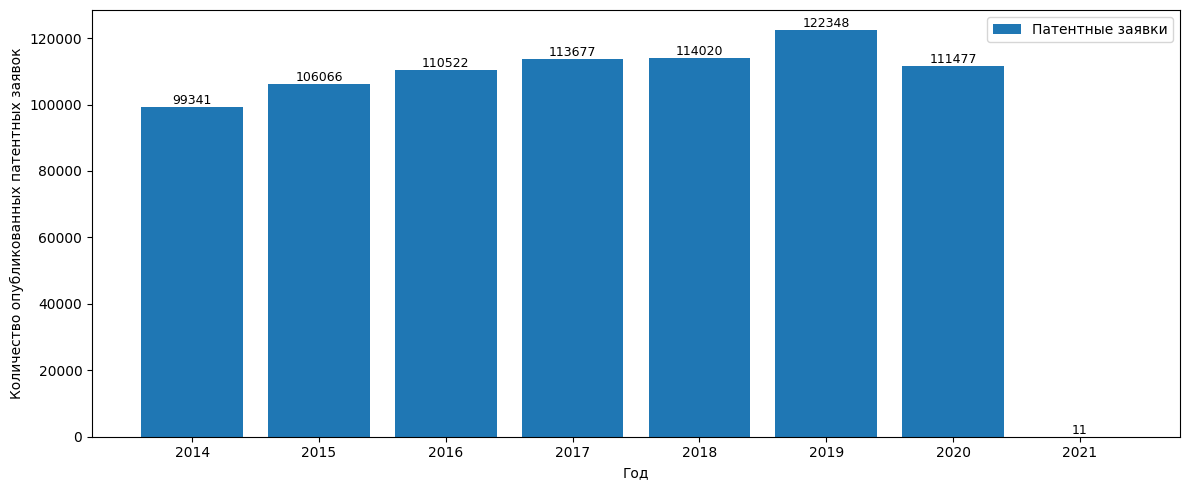
\includegraphics[width=0.95\linewidth]{figures/years_hist.png}
\caption{Распределение патентов по году публикации (2014--2021)}
\label{fig:year_dist}
\end{figure}

Для дальнейшего исследования в качестве \textbf{генеральной совокупности} была выбрана наиболее актуальная часть массива --- \textbf{``свежие'' патенты}, опубликованные начиная с \textbf{2020-01-01}. Такой подход соответствует практической задаче мониторинга и прогнозирования патентного ландшафта: именно новые публикации в наибольшей степени отражают текущие технологические тренды, появление развивающихся направлений и изменения на границах технических областей.

В результате применения временного фильтра была сформирована генеральная совокупность объёмом \textbf{111\,479} патентных документов, которая использовалась в последующих этапах анализа (построение эмбеддингов, снижение размерности, визуализация и проверка гипотезы о согласованности семантического пространства с технологической классификацией).

На рисунке~\ref{fig:cpc_sections} показано распределение \textbf{главных семейств CPC} (по первой букве секции) для сформированной генеральной совокупности патентных документов. Диаграмма отражает доминирующие технологические направления и позволяет выбрать приоритетные области для дальнейшего анализа и визуализации.

\begin{figure}[h]
\centering
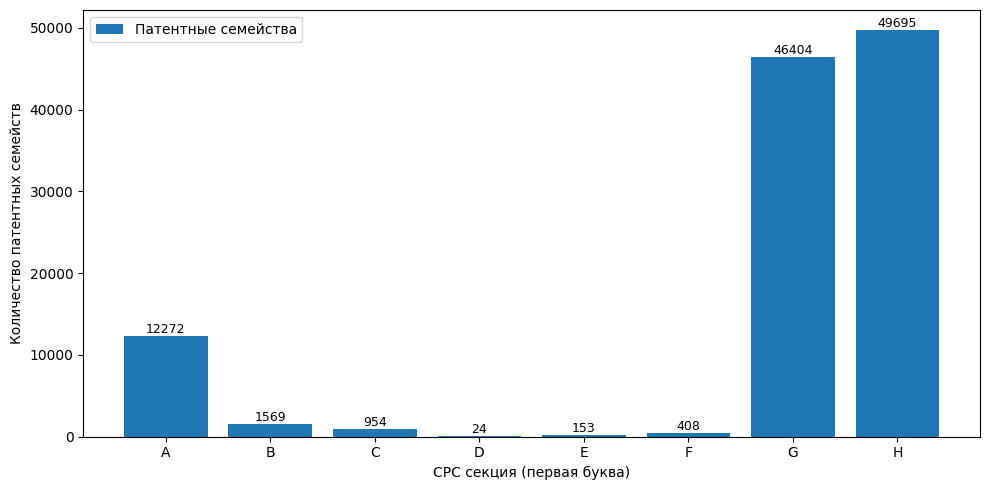
\includegraphics[width=0.95\linewidth]{figures/cpc_fam_hsit.png}
\caption{Распределение патентных документов по секциям CPC в генеральной совокупности}
\label{fig:cpc_sections}
\end{figure}

Система CPC (Cooperative Patent Classification) делит изобретения на 8 базовых секций, обозначаемых буквами:
\begin{itemize}
  \item \textbf{A} --- \textit{Human necessities}: медицина, гигиена, сельское хозяйство, пищевые продукты, предметы быта и т.п.
  \item \textbf{B} --- \textit{Performing operations; Transporting}: обработка материалов, технологические операции, упаковка, транспортировка.
  \item \textbf{C} --- \textit{Chemistry; Metallurgy}: химия, материалы, полимеры, фармацевтика, металлургия.
  \item \textbf{D} --- \textit{Textiles; Paper}: текстиль, бумага, соответствующие технологии производства.
  \item \textbf{E} --- \textit{Fixed constructions}: строительство, сооружения, горные работы.
  \item \textbf{F} --- \textit{Mechanical engineering; Lighting; Heating; Weapons; Blasting}: машиностроение, двигатели, отопление, освещение, вооружение.
  \item \textbf{G} --- \textit{Physics}: измерения, вычисления, оптика, управление, коммуникации (на уровне физики/приборов).
  \item \textbf{H} --- \textit{Electricity}: электротехника, электроника, телекоммуникации, вычислительная техника и смежные области.
\end{itemize}

В дальнейшем для более детального анализа будет рассмотрено одно из наиболее объёмных семейств --- \textbf{H (Electricity)}. Выбор данного семейства обусловлен его высокой представленностью в генеральной совокупности и практической значимостью для задач мониторинга технологических трендов в области электроники и электротехники.

На рисунке~\ref{fig:h_subfamilies} показано распределение \textbf{подсемейств} выбранной группы (например, по атрибуту \texttt{main\_cpc\_fam}) и их относительный вклад в общий объём патентов семейства H.

\begin{figure}[h]
\centering
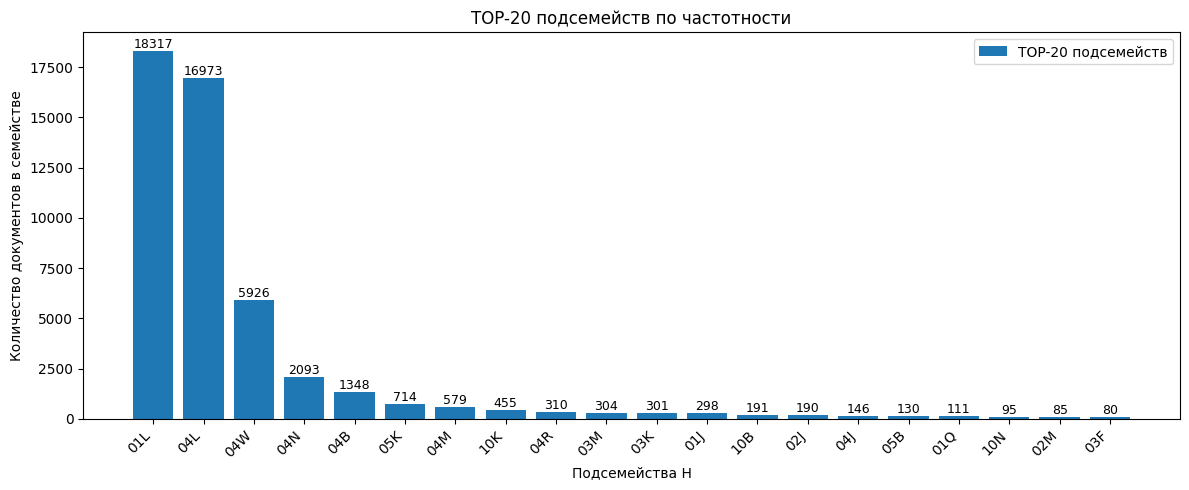
\includegraphics[width=0.95\linewidth]{figures/cpc_subfam_hist.png}
\caption{Распределение подсемейств CPC внутри семейства H}
\label{fig:h_subfamilies}
\end{figure}


\subsection{Применение алгоритма PCA}
Для снижения вычислительной нагрузки и повышения удобства последующего анализа была применена редукция размерности методом \textbf{PCA} (Principal Component Analysis). В рамках предварительного этапа выполнено аналитическое исследование \textbf{кумулятивной объяснённой дисперсии} для исходных эмбеддингов: было оценено, какая доля вариативности данных сохраняется при выборе различного числа главных компонент. Ключевые рубежные значения (пороги сохранённой дисперсии) отмечены на графике, представленном на рисунке~\ref{fig:pca_cumvar}.

\begin{figure}[h]
\centering
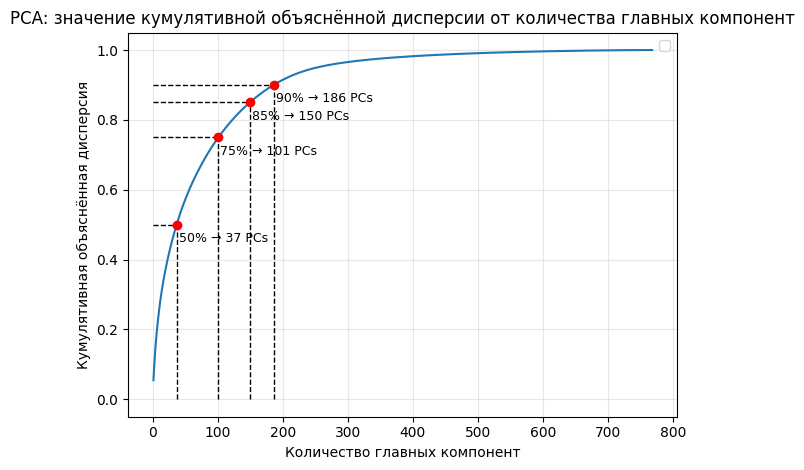
\includegraphics[width=0.75\linewidth]{figures/PCA_com.png}
\caption{Кумулятивная объяснённая дисперсия PCA в зависимости от числа компонент}
\label{fig:pca_cumvar}
\end{figure}

По результатам анализа было выбрано такое число компонент, при котором сохраняется \textbf{90\%} дисперсии выборки: для этого потребовалось \textbf{186} главных компонент. Таким образом, размерность признакового пространства была уменьшена более чем в \textbf{4 раза} по сравнению с исходной (768), что позволяет существенно ускорить вычисления при сохранении основной части информации, содержащейся в эмбеддингах.

\subsection{t-SNE (визуализация)}
Для проверки того, насколько семантические эмбеддинги отражают \textbf{локальную смысловую структуру} патентных документов, была выполнена визуализация методом \textbf{t-SNE}. В качестве целевой области рассмотрено CPC-семейство \textbf{H (Electricity)}, а также выбраны наиболее представленные подсемейства для последующего сравнения их пространственного распределения.

На рисунке~\ref{fig:tsne_top15} приведены результаты визуализации для \textbf{15 наиболее частотных подсемейств} семейства H. Точки раскрашены по подсемействам, в легенде дополнительно указано количество патентных документов в каждом классе.

\begin{figure}[h]
\centering
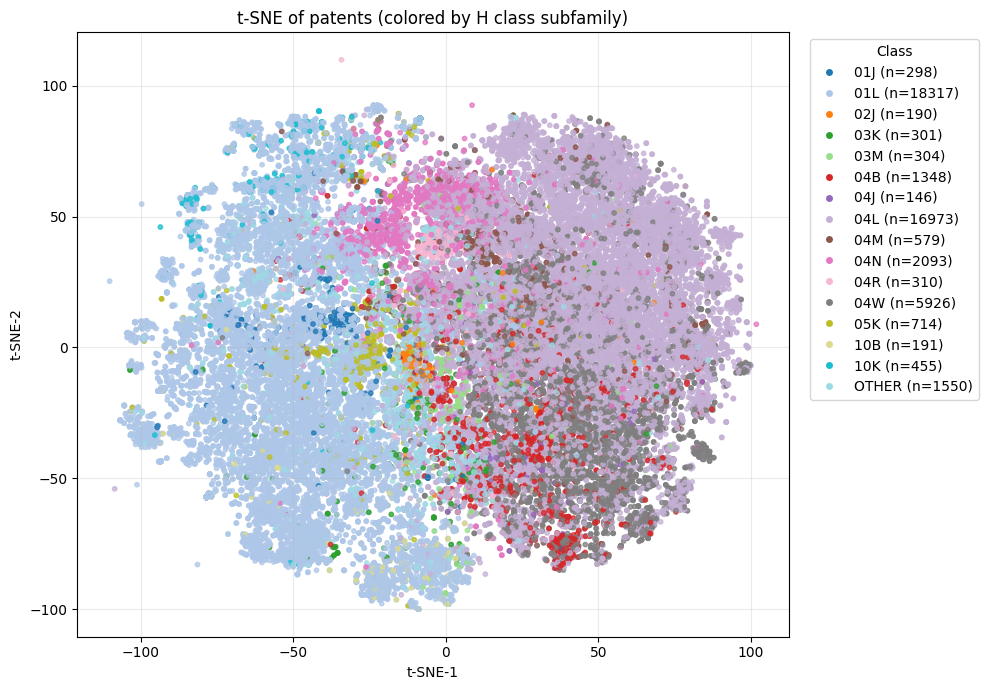
\includegraphics[width=0.95\linewidth]{figures/tsne_b.png}
\caption{t-SNE-визуализация патентов семейства H для 15 наиболее частотных подсемейств (в легенде указано число документов)}
\label{fig:tsne_top15}
\end{figure}

Как видно из рисунка~\ref{fig:tsne_top15}, t-SNE демонстрирует \textbf{чёткое биполярное разделение} пространства эмбеддингов: наблюдаются две плотные области, визуально различимые друг от друга, и \textbf{зона перекрытия} в центральной части. При этом t-SNE корректнее интерпретировать именно на уровне \textbf{локальных соседств}: близко расположенные точки соответствуют семантически близким названиям патентов, тогда как глобальные расстояния и взаимное расположение крупных ``облаков'' в 2D проекции не всегда отражают реальные расстояния в исходном пространстве.

Наблюдаемая структура указывает, что семейство \textbf{H (Electricity)} не является семантически однородным и распадается как минимум на \textbf{два крупных подпространства}. Вероятно, выделяемые области отражают различия между \textbf{аппаратно-ориентированными} и \textbf{системно-сетевыми} технологиями внутри семейства H. Зона перекрытия может свидетельствовать о наличии патентов \textbf{смешанного характера}, сочетающих аппаратные и системные аспекты, что является характерным признаком междисциплинарности современных электротехнических решений.

Кроме того, из-за выраженного дисбаланса классов крупные подсемейства могут визуально ``подавлять'' менее представленные группы. Чтобы снизить влияние этого эффекта и проверить устойчивость наблюдаемой картины, была выполнена вторая визуализация: рассмотрены \textbf{20 наиболее частотных подсемейств}, при этом для каждого подсемейства выполнена равномерная выборка (не более заданного числа объектов на класс). Результаты приведены на рисунке~\ref{fig:tsne_sampled}.

\begin{figure}[h]
\centering
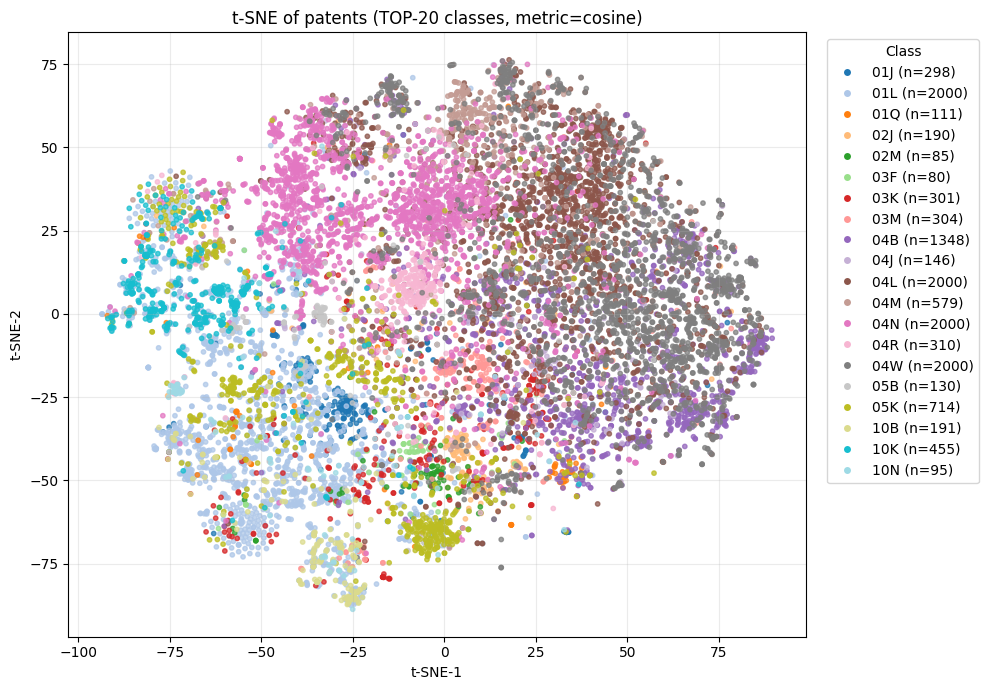
\includegraphics[width=0.95\linewidth]{figures/tsne_s.png}
\caption{t-SNE-визуализация патентов семейства H для 20 наиболее частотных подсемейств при ограничении числа объектов на класс}
\label{fig:tsne_sampled}
\end{figure}

Во второй визуализации использовано ограничение числа объектов на класс (до 2000), что уменьшает эффект доминирования крупнейших подсемейств и позволяет лучше рассмотреть структуру менее представленных групп. Полученная t-SNE-проекция демонстрирует следующие особенности:

\begin{itemize}
  \item \textbf{Устойчивость макроструктуры:} после балансировки сохраняется крупномасштабная организация пространства (выраженные плотные области и центральная зона смешения). Это указывает на то, что наблюдаемая структура не является артефактом дисбаланса и проявляется на уровне локальной семантики эмбеддингов.
  \item \textbf{Различимость подсемейств на локальном уровне:} часть подсемейств формирует достаточно \textbf{компактные ``острова''} (локальные кластеры), что соответствует ожиданию: близкие по смыслу названия патентов оказываются соседями в embedding-пространстве.
  \item \textbf{Зоны перекрытия и размытые границы:} в центральной области заметно \textbf{смешение цветов} — ряд подсемейств существенно перекрываются. Это может означать как тематическую близость (общая терминология и пересечение предметных областей), так и то, что по одному лишь названию патента не всегда удаётся однозначно разделить классы на выбранном уровне детализации.
  \item \textbf{Неоднородность семейства H:} общая картина подтверждает предположение о том, что семейство H не является семантически единым: внутри него существуют несколько крупных областей, связанные ``переходными'' зонами. Такие переходные области можно интерпретировать как патенты смешанного характера, сочетающие признаки разных направлений.
\end{itemize}

В совокупности рисунок~\ref{fig:tsne_sampled} служит качественной иллюстрацией того, что эмбеддинги отражают локальную структуру и показывают как зоны чёткой тематической концентрации, так и области междисциплинарного пересечения, которые потенциально важны для задач мониторинга и анализа патентного ландшафта.

\subsection{kNN (количественная проверка гипотезы)}
Для количественной проверки гипотезы H1 был выбран подход, основанный на \textbf{анализе ближайших соседей} в пространстве эмбеддингов. Идея теста заключается в следующем: если семантические представления действительно согласуются с технологической классификацией, то для каждого патента его ближайшие соседи (по косинусной близости) должны чаще принадлежать к тому же CPC-подсемейству, а простой классификатор на основе соседей должен давать качество существенно выше базовых предположений.

Проверка выполнялась с использованием \textbf{kNN-классификатора} с косинусной метрикой и взвешиванием вкладов соседей по расстоянию. Для получения устойчивой оценки качества и исключения переобучения применялась \textbf{стратифицированная кросс-валидация} (5-fold Stratified CV), обеспечивающая сохранение пропорций классов в каждом фолде. Процедура включала следующие шаги:
\begin{enumerate}
  \item Данные разбивались на 5 непересекающихся фолдов так, чтобы распределение CPC-подсемейств в каждом фолде было близким к исходному.
  \item Для каждой итерации кросс-валидации 4 фолда использовались как обучающая выборка: для каждого объекта из тестового фолда классификатор находил заданное число ближайших соседей среди обучающих объектов в пространстве эмбеддингов.
  \item Класс тестового объекта определялся по \textbf{взвешенному голосованию} соседей: более близкие объекты оказывали больший вклад в итоговое решение.
  \item После завершения всех 5 итераций формировались out-of-fold предсказания для всех объектов и вычислялись метрики качества.
\end{enumerate}

Для оценки гипотезы использовались следующие показатели:
\begin{itemize}
  \item \textbf{Accuracy} --- доля правильных предсказаний. Метрика отражает общее качество, но чувствительна к дисбалансу классов.
  \item \textbf{Macro-F1} --- среднее F1 по классам (каждый класс имеет одинаковый вес), что позволяет оценить качество на редких подсемействах.
  \item \textbf{Top-5 accuracy} --- доля случаев, когда истинный класс присутствует среди классов $k$ ближайших соседей. Эта метрика ближе к практическим сценариям \textbf{семантического поиска и рекомендаций}, когда важно, чтобы правильный класс находился среди ближайших кандидатов, а не обязательно был первым.
\end{itemize}

Дополнительно результаты сравнивались между двумя вариантами признакового пространства: \textbf{исходными эмбеддингами} и их \textbf{редуцированным представлением} после PCA. Такое сравнение позволяет оценить, насколько снижение размерности сохраняет локальную структуру соседств, необходимую для классификации и поиска.

\newpage
\section{Результаты}
\subsection{Сравнение kNN-метрик (5-fold CV)}
\begin{table}[h]
\centering
\caption{Метрики kNN (mean$\pm$std) при 5-fold CV}
\begin{tabular}{lccc}
\toprule
\textbf{Представление} & \textbf{Accuracy} & \textbf{Macro-F1} & \textbf{Top-5 accuracy} \\
\midrule
PatentSBERTa (768) & 0.7920 $\pm$ 0.0026 & 0.4449 $\pm$ 0.0076 & 0.9268 $\pm$ 0.0015 \\
PCA-186            & 0.7910 $\pm$ 0.0027 & 0.4431 $\pm$ 0.0066 & 0.9257 $\pm$ 0.0021 \\
\bottomrule
\end{tabular}
\end{table}

\textbf{Интерпретация:} различия между 768 и PCA-186 минимальны (порядка $10^{-3}$), следовательно, PCA-редукция \textbf{почти не ухудшает} локальные соседства и качество kNN-классификации.

\subsection{Сводные метрики по \texttt{classification\_report}}
Для более детального анализа построен \texttt{classification\_report} (out-of-fold предсказания). Сводные строки приведены в таблице~\ref{tab:summary}.

\begin{table}[h]
\centering
\caption{Сводные метрики \texttt{classification\_report} (TOP-15)}
\label{tab:summary}
\begin{tabular}{lcccc}
\toprule
\textbf{Представление} & \textbf{Accuracy} & \textbf{Macro P/R/F1} & \textbf{Weighted P/R/F1} \\
\midrule
768 & 0.7920 & 0.6234 / 0.3807 / 0.4458 & 0.7745 / 0.7920 / 0.7735 \\
PCA-186 & 0.7910 & 0.6185 / 0.3806 / 0.4437 & 0.7734 / 0.7910 / 0.7724 \\
\bottomrule
\end{tabular}
\end{table}

\textbf{Бейзлайн по большинству (majority class):} если всегда предсказывать самый частый класс 01L, точность составит
\[
\text{Acc}_{maj} = \frac{18317}{48145} \approx 0.3805.
\]
Следовательно, kNN даёт \textbf{существенный выигрыш} по сравнению с наивным классификатором, что поддерживает гипотезу о наличии информации о CPC-классах в семантических эмбеддингах.

\subsection{Поклассовые метрики (768)}
\begin{table}[h]
\centering
\caption{Поклассовые метрики kNN (cosine) для 768-мерных эмбеддингов}
\scriptsize
\begin{tabular}{lcccc}
\toprule
\textbf{Класс} & \textbf{Precision} & \textbf{Recall} & \textbf{F1} & \textbf{Support} \\
\midrule
01J & 0.6885 & 0.2819 & 0.4000 & 298 \\
01L & 0.8970 & 0.9724 & 0.9332 & 18317 \\
02J & 0.6577 & 0.3842 & 0.4850 & 190 \\
03K & 0.6833 & 0.1362 & 0.2271 & 301 \\
03M & 0.7267 & 0.3586 & 0.4802 & 304 \\
04B & 0.5478 & 0.2634 & 0.3557 & 1348 \\
04J & 0.5000 & 0.1096 & 0.1798 & 146 \\
04L & 0.7633 & 0.8691 & 0.8127 & 16973 \\
04M & 0.6696 & 0.2660 & 0.3807 & 579 \\
04N & 0.7217 & 0.4845 & 0.5798 & 2093 \\
04R & 0.7188 & 0.5935 & 0.6502 & 310 \\
04W & 0.6003 & 0.5511 & 0.5746 & 5926 \\
05K & 0.6350 & 0.2997 & 0.4072 & 714 \\
10B & 0.1724 & 0.0262 & 0.0455 & 191 \\
10K & 0.3688 & 0.1143 & 0.1745 & 455 \\
\bottomrule
\end{tabular}
\end{table}

\subsection{Поклассовые метрики (PCA-186)}
\begin{table}[h]
\centering
\caption{Поклассовые метрики kNN (cosine) для PCA-186}
\scriptsize
\begin{tabular}{lcccc}
\toprule
\textbf{Класс} & \textbf{Precision} & \textbf{Recall} & \textbf{F1} & \textbf{Support} \\
\midrule
01J & 0.6829 & 0.2819 & 0.3990 & 298 \\
01L & 0.8968 & 0.9719 & 0.9329 & 18317 \\
02J & 0.6102 & 0.3789 & 0.4675 & 190 \\
03K & 0.7407 & 0.1329 & 0.2254 & 301 \\
03M & 0.6727 & 0.3651 & 0.4733 & 304 \\
04B & 0.5542 & 0.2656 & 0.3591 & 1348 \\
04J & 0.4839 & 0.1027 & 0.1695 & 146 \\
04L & 0.7623 & 0.8682 & 0.8118 & 16973 \\
04M & 0.6638 & 0.2660 & 0.3798 & 579 \\
04N & 0.7197 & 0.4845 & 0.5791 & 2093 \\
04R & 0.7393 & 0.6129 & 0.6702 & 310 \\
04W & 0.5975 & 0.5466 & 0.5709 & 5926 \\
05K & 0.6265 & 0.2913 & 0.3977 & 714 \\
10B & 0.1667 & 0.0262 & 0.0452 & 191 \\
10K & 0.3611 & 0.1143 & 0.1736 & 455 \\
\bottomrule
\end{tabular}
\end{table}

\newpage
\section{Анализ результатов и выводы}
\subsection{Ключевые наблюдения}
\begin{itemize}
  \item \textbf{Подтверждение гипотезы H1:} kNN-классификация по эмбеддингам показывает высокую точность (accuracy $\approx 0.79$), а top-5 accuracy $\approx 0.926$, что указывает на сильную согласованность \textbf{локального соседства} с CPC-подсемействами.
  \item \textbf{PCA-186 сохраняет качество:} разница между 768 и PCA-186 минимальна по всем ключевым метрикам (accuracy, macro-F1, top-5), значит PCA практически не разрушает семантическую структуру, полезную для kNN.
  \item \textbf{Влияние дисбаланса:} macro recall $\approx 0.38$ и macro-F1 $\approx 0.44$ заметно ниже accuracy. Это означает, что качество на \textbf{редких классах} существенно хуже, чем на крупных.
  \item \textbf{Лучше всего распознаются крупные подсемейства:} 01L (F1 $\approx 0.93$) и 04L (F1 $\approx 0.81$) демонстрируют стабильное качество; для малых классов (например, 10B) качество крайне низкое (F1 $\approx 0.045$), что согласуется с малым числом примеров и вероятными зонами смешения в t-SNE.
  \item \textbf{Сильный выигрыш относительно бейзлайна:} majority baseline $\approx 0.3805$, тогда как kNN достигает $\approx 0.792$, что подтверждает наличие существенного сигнала CPC-класса в эмбеддингах.
\end{itemize}

\subsection{Итоговые выводы}
\begin{enumerate}
  \item Эмбеддинги PatentSBERTa по \textbf{названиям} патентов семейства H содержат выраженную информацию о CPC-подсемействах и поддерживают семантическую близость документов в соответствии с технологической разметкой.
  \item Снижение размерности до \textbf{PCA-186} почти не снижает качество, поэтому подходит для ускорения расчётов и визуализации в программной системе анализа патентов.
  \item Существенное ограничение подхода --- \textbf{дисбаланс классов} и слабое качество на редких подсемействах; для улучшения могут потребоваться балансировка данных, объединение уровней CPC или использование более информативных текстовых полей (аннотация/claims).
\end{enumerate}

\newpage
\begin{thebibliography}{99}

\bibitem{uspto}
United States Patent and Trademark Office (USPTO) (Ведомство по патентам и товарным знакам США): офиц. сайт. --- Текст: электронный. --- Режим доступа: \texttt{https://www.uspto.gov/} (дата обращения: ноябрь 2025).

\bibitem{patentsberta}
Bekamiri H., Hain D.\,S., Jurowetzki R. PatentSBERTa: A Deep NLP based Hybrid Model for Patent Distance and Classification using Augmented SBERT: препринт. --- Текст: электронный // arXiv. --- 2021. --- arXiv:2103.11933. --- Режим доступа: \texttt{https://arxiv.org/abs/2103.11933} (дата обращения: ноябрь 2025).

\bibitem{sklearn}
scikit-learn: Machine Learning in Python: документация. --- Текст: электронный. --- Режим доступа: \texttt{https://scikit-learn.org/stable/} (дата обращения: декабрь 2025).

\end{thebibliography}


\end{document}

